\documentclass[11pt]{book}
\usepackage{geometry}        
\geometry{letterpaper}    
\usepackage[parfill]{parskip}  
\usepackage{graphicx}
\usepackage{caption}
\usepackage{subcaption}
\usepackage{amssymb}
\usepackage{epstopdf}
\usepackage{listings}
\usepackage{times}
\usepackage{float}

\usepackage{cleveref}

\usepackage[final]{pdfpages}

\AtBeginDocument{\renewcommand{\bibname}{References}}
\DeclareGraphicsRule{.tif}{png}{.png}{`convert #1 `dirname #1`/`basename #1 .tif`.png}

\usepackage[colorlinks=true, pdfstartview=FitV, linkcolor=black, 
            citecolor=blue, urlcolor=blue]{hyperref}

\usepackage{tocloft}



\renewcommand\cftchapfont{\Large\bfseries}
\renewcommand\cftsecfont{\Large\bfseries}

%\renewcommand\cftchappagefont{\LARGE\bfseries}
%\renewcommand\cftsecpagefont{\LARGE}

\renewcommand\cftchapafterpnum{\par\addvspace{6pt}}
\renewcommand\cftsecafterpnum{\par\addvspace{6pt}}

% ------------------- Title and Author -----------------------------

\setlength\parindent{24pt}
\renewcommand{\baselinestretch}{1}
\linespread{1.5}

\begin{document}

\begin{titlepage}
    \begin{center}
                
        \Large
        \textbf{A Shiny App for Introductory Statistics Concepts}
        
      
        \vspace{1cm}
       
        
        \Large
        Chelsey Legacy \\
        \vspace{0.25cm}
        Department of Statistics\\
          \vspace{0.25cm}
        Iowa State University\\
       
        
        \vspace{1cm}
               
           Creative Component\\
             \vspace{0.25cm}
           Spring 2017
           
           \vspace{2cm}
         
				\begin{center}
				\begin{tabular}{rl}
				Committee Members: & Amy G. Froelich, Major Professor\\
				 & W. Robert Stephenson \\
				 & Heike Hofmann\\
				\end{tabular}
				\end{center}
           
    \end{center}
\end{titlepage}







\begin{center}
\textbf{Abstract}
\end{center}
Technology has become an essential part of teaching an introductory statistics course. Research has shown that technology has the ability to further students conceptual knowledge in addition to assisting in calculations. Though there are many different software options available to serve this purpose, this paper focuses on R's Shiny app. Shiny apps can be customized and made available to students on any browser at no cost to the students. A Shiny app was created focusing on the basics of topics such as: inference for one and two proportions, inference for one and two means, linear regression, and ANOVA. Ancillary worksheets were created pertaining to each of the topics covered. Future work will go into getting feedback on the Shiny app and its ability to aid in learning concepts.

\newpage
\tableofcontents
\renewcommand\thechapter{\arabic{chapter}}
\renewcommand\thesection{\arabic{section}}
%\renewcommand\thesubsection{(\arabic{subsection})}

\newpage
\section{Introduction}
Over the past 30 years, technology has become an integral part of teaching undergraduate statistics courses. Statistical software packages like JMP, StatCrunch, R, and Minitab are used to teach students the skills to conduct data analysis. Some of these same programs plus Java web-based applets have been used to teach students concepts in introductory statistics, particularly sampling distributions and inferential topics. Instructors select technology platforms based on a number of concerns particular to their audience and institution. One recent option, R's Shiny applications, provides an easy to use and interactive interface for introductory statistics students. The application can run on any web browser, allowing students and instructors to use the app on mobile devices, tablets, Chromebooks, and computers, with no cost to the students or instructor. As a relatively new option for instructional technology, there are few resources available for the introductory statistics course using the Shiny application in R. In this paper, we will outline the creation of an R shiny app and supporting supplemental worksheets to be used in conjunction with the app for the introductory statistics course. The Shiny app includes resources for teaching concepts in inference for a population proportion, population mean, difference between two population proportions, and the difference between two population means; descriptive linear regression and correlation, and ANOVA.

In section 2, we will discuss the literature related to technology in the classroom, specifically as it relates to teaching concepts in introductory statistics. In section 3, the development of the Shiny app is detailed, and we discuss the supplemental worksheets in Section 4. Conclusions and details of future work appear in Section 5.
 
\section{Literature Review}
	   	
	Most undergraduate statistics courses make use of some sort of technology in the classroom, from calculators to computer software programs. Using technology allows instructors to simplify complex calculations and make conceptual ideas more concrete. In this way, the technology used in the statistics classroom is an example of a cognitive technology - ``any medium that helps transcend the limitations of the mind (e.g. attention to goals, short-term memory span), in thinking, learning, and problem-solving activities" (Pea, 1987, p. 91). Cognitive technologies ``make external the intermediate products of thinking $\ldots$, which can then be analyzed, reflected upon, and discussed" (Pea, 1987, p. 91). With the help of computers, we are able to put thoughts and equations into visual and graphical representations that can then be viewed by many and discussed in an effort to clarify statistical concepts. Computer applets and software are precisely the type of cognitive technologies being described that can help student thinking to go beyond just following formulas and returning answers.  Pea summarizes this idea by stating, ``the dynamic and interactive media provided by computer software make gaining an intuitive understanding (traditionally the province of the professional mathematician) of the interrelationships among graphic, equational, and pictorial representations more accessible to the software user."(1987, p. 96)  
		
The use of cognitive technologies in the classroom has had a profound impact on the pedagogy of statistics. Chance, Ben-Zvi, Garfield, \& Medina (2007) discuss how courses are changing format in response to these technologies. They specify that, "students are evaluated less on their ability to manipulate formulas and look up critical values, and more on their ability to select appropriate tools (e.g., choosing techniques based on the variables involved), assess the validity of different techniques, utilize graphical tools for exploration of data, deal with messier data sets, provide appropriate interpretations of computer output, and evaluate and communicate the legitimacy of their conclusions" (Chance, et. al, 2007, p. 3).  They state, "technology has expanded the range of graphical and visualization techniques to provide powerful new ways to assist students in exploring and analyzing data and thinking about statistical ideas, allowing them to focus on interpretation of results and understanding concepts rather than computational mechanics" (Chance, et. al, 2007, p. 3). Although technology has many benefits, it is important that the technology should support the course learning objectives, and not restructure the objectives to pertain to learning the software.  Chance et. al (2007) argue that technology should not be used ``merely for the sake of using technology",  but instead used for accessing, analyzing and interpreting large real data sets, automating calculations and processes, generating and modifying appropriate statistical graphics and models, performing simulations to illustrate abstract concepts and exploring 'what happens if...' type questions" (Chance, et. al, 2007, p. 2-3).

There are increasingly many different software programs and applets available to supplement introductory statistics courses. ``(T)he types of technology used in statistics and probability instruction can be broken into several categories: Statistical software packages, educational software, spreadsheets, applets/standalone applications, graphing calculators, multimedia materials, and data repositories." (Chance, et. al, 2007, p. 4). Instructors choose among these various options based on the content of their course, their selected course materials including textbooks, their students expected competency on such programs, and funding availability. To avoid the course becoming inaccessible to those students, the software chosen should be fairly straightforward and require no previous knowledge. Use of complex programs provides the problem of the students focusing so much on learning the software that they lose sight of the statistical concepts they are actually supposed to be learning. 

For statistical software packages, Fathom, Minitab, and JMP are all point-and-click programs that allow users to enter and manipulate data, obtain graphical and summary statistics of the data, and fit a variety of different statistical models. Only basic computer skills are needed to learn these programs, and no programming experience is necessary. However, the main drawback of these programs is cost, either to the institution or to the students. The freely available program R (also through R Studio) can provide the same statistical analyses needed by the students. However, the learning curve for both instructors and students tends to be steeper with R than with other programs. In addition to software, there are a large number of freely available web-based Java applets that provide conceptual frameworks for simulations, p-values, and other intro stat concepts (for example, Rossman and Chance (2004)). These are helpful additions to lecture slides and materials; however, no supplemental materials are provided that can help guide student interaction with the applets. While there are a multitude of available software and programs, eventually an instructor may have difficulty finding an applet or software that perfectly suits their needs for teaching and student learning (Doi, Potter, Wong, Alcaraz, \& Chi, 2016).  

With monetary and time costs to consider, R's Shiny app technology has several advantages for use in the classroom. With this technology, the developer can create an interactive app that is point and click based, and allows the user to perform complex tasks with the click of a button.  The user never has to engage in writing or seeing the code unless the developer so chooses.  The developer is the only one that must have a basic understanding of coding in R to successfully create the app (Doi, et. al., 2016). After creation and publication to the web, students can easily interact with the app from a web browser from phones, tablets, and computers. This allows the technology to be used by all students in classrooms other than just computer classrooms, which is appealing to lectures without access to computer classrooms. In addition, the ease of design of a Shiny app allows it to be "especially helpful when teaching concepts that are not in the standard curriculum or based on recent research" (Doi, et. al., p 6). Newer concepts may not already have applets or software available for classroom demonstrations, thus Shiny can be used to create something to fill this gap. It could also be used to create tailor made lecture materials for a specific course. Apps can be created based on the different topics in that course and thus creating a collection of relevant tools for a corresponding course. Technologies such as R's Shiny web applications have the ability to provide insights to students through their interactivity and the output they provide that are not available through lectures or notes on a blackboard.
 
 
 % ------------------------------Shiny Web App Sections ---------------------------%

\section{Shiny Web Application Design}
The main goal of this project was to create a Shiny app to help introductory statistics students gain some insight and confidence in working with complex concepts. There are many different concepts introduced to students in introductory statistics courses.  A few of these concepts were chosen to be the focus of the Shiny app.  The topics of focus are inference for one and two sample proportions, inference for one and two means, linear regression, and ANOVA.  The Shiny app is composed of several tabs, each dedicated to one of these topics. Using the Shiny reference and examples pages, a design was planned out for each of the different sections. Then, the applications were programmed for each section and subsection. 


\subsection{One Proportion: Sampling Distribution}
As seen in Figure \ref{fig:OneProp} the Shiny app opens up to the sampling distribution for one sample proportion. This section is designed to help enhance student comprehension of the difference between a sample distribution and sampling distribution for a sample proportion. At the top of the application a variety of variables such as sample size, number of samples, and population proportion can be manipulated. Once these are set, the user can hit the "Draw" button and the application will perform the simulation. 

The sample distribution graph is created using a binomial distribution with the proportion and sample size input by the user. If only one sample is created, the Sampling Distribution graph will only display the sample proportion from this one sample. If the user chooses to draw more than one sample, the Sample Distribution graph will display the last sample drawn and the Sampling Distribution will show the histogram of all sample proportions generated from the samples. The tables in the middle of the page provide summary information about the Sample and Sampling Distributions. The Sample Summary Statistics shows a relative frequency table for the last sample drawn, while the Summary Sampling Distribution Statistics display the mean and standard deviation of the Sampling Distribution. 

\subsection{One Proportion: Confidence Intervals}
The next section under the inference for one proportion is designed to demonstrate the effects of confidence level and sample size on the construction of confidence intervals, as seen in Figure \ref{fig:OnePropCI}. The user can manipulate the sample size and the confidence level as sliders, with the confidence level ranging from 80 to 99 percent and the sample size ranging from 25 to 500. The sample size allows for values from 25 to 500.  The graph automatically displays 20 confidence intervals, created using 20 sample proportions drawn from a binomial with $p= 0.5$, the input sample size, and $80\%$ confidence level. The lines represent the different confidence intervals and are colored according to whether or not they captured the true population parameter, 0.5.  Light blue lines represent the confidence intervals that contained 0.5, while the orange lines represent those that did not contain 0.5. 

\begin{figure}
        \centering

        \begin{subfigure}[b]{0.75\textwidth}
                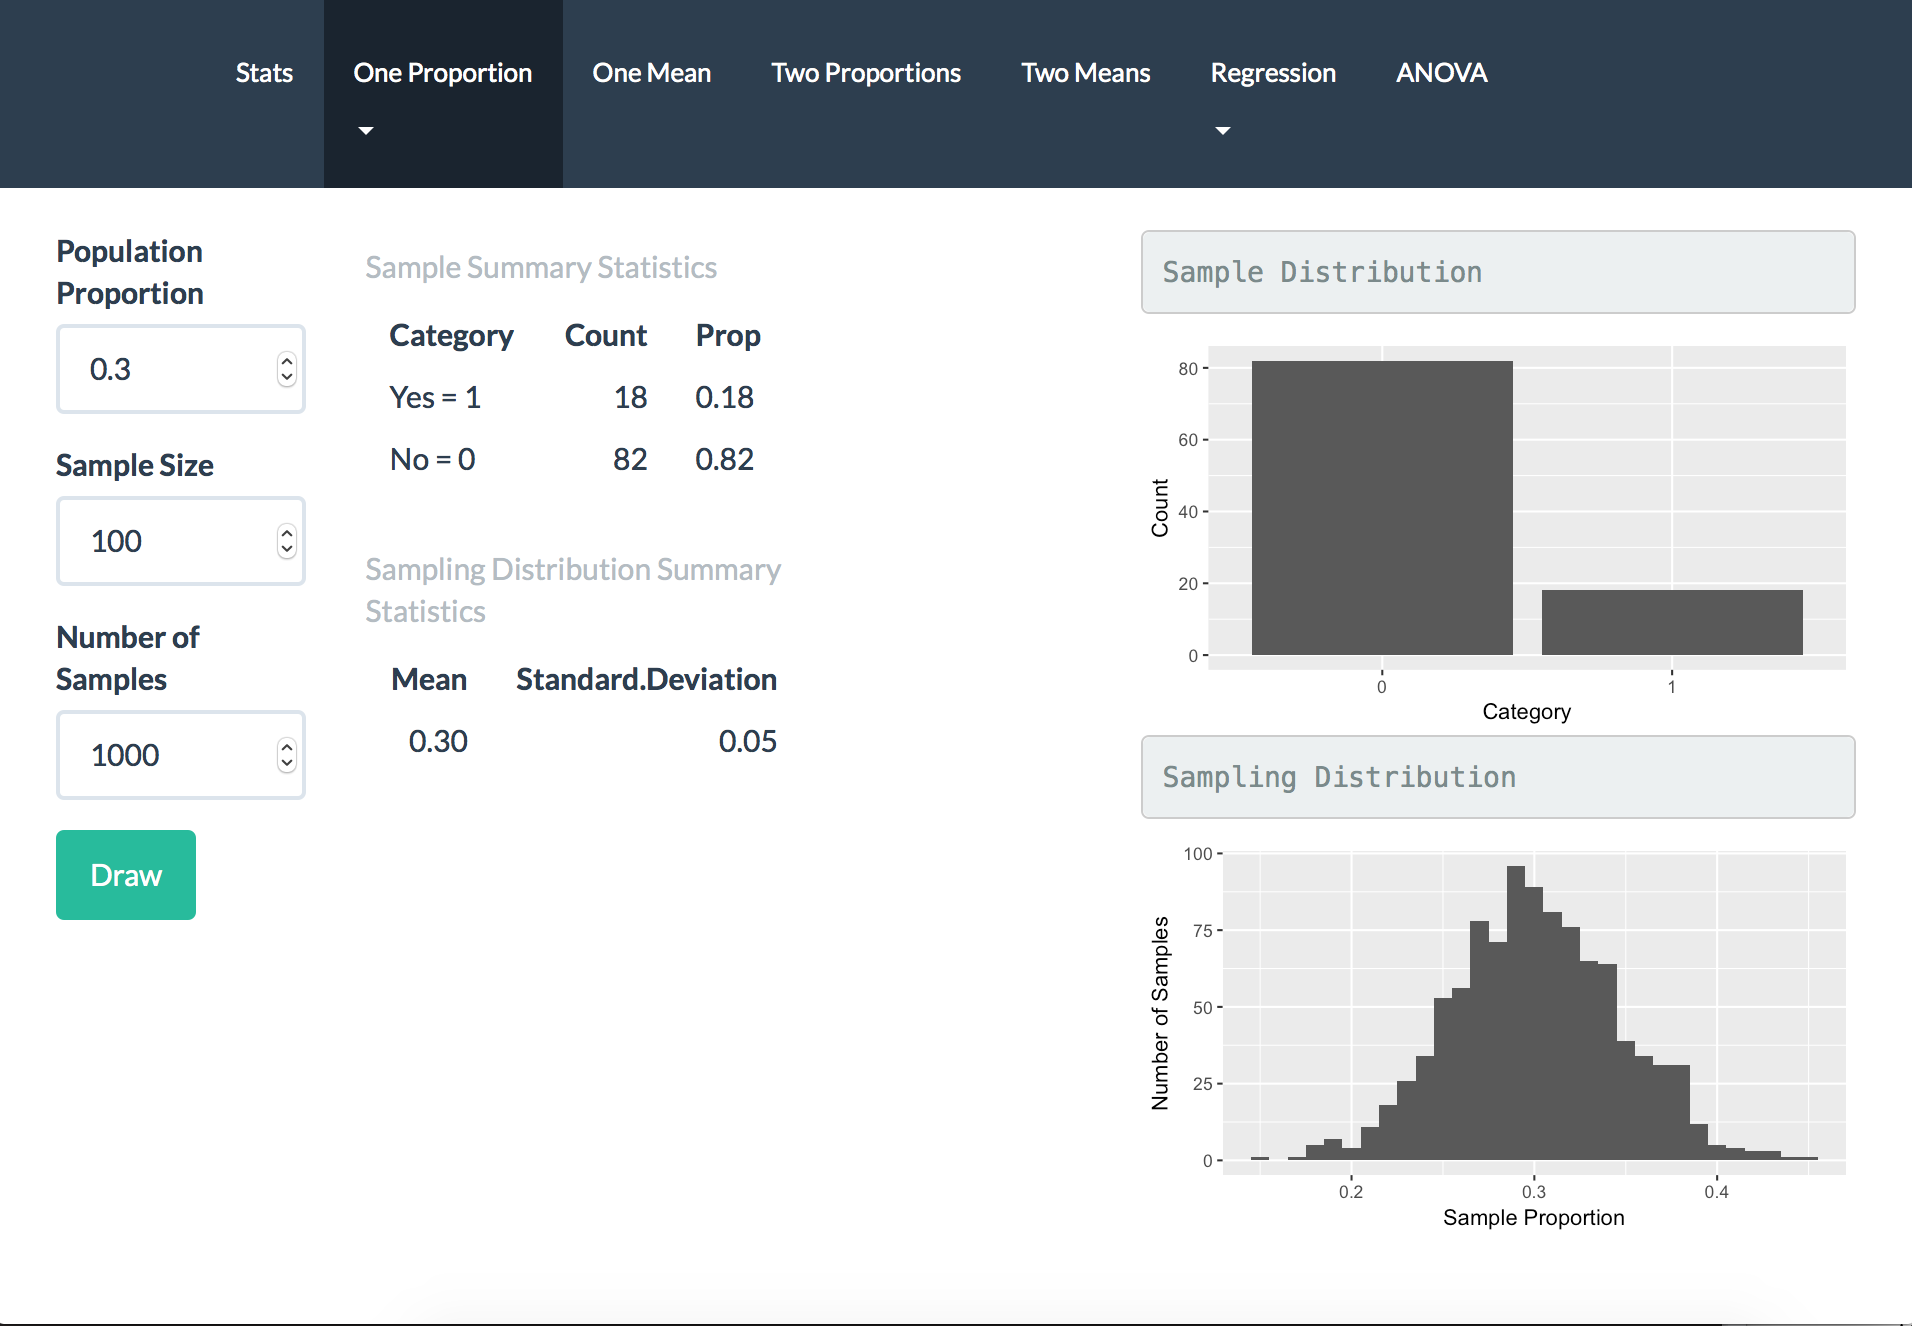
\includegraphics[width=\textwidth]{OneProp.png}
                \caption{Sampling Distribution Screen }
                \label{fig:OneProp}
        \end{subfigure}%

        \begin{subfigure}[b]{0.75\textwidth}
                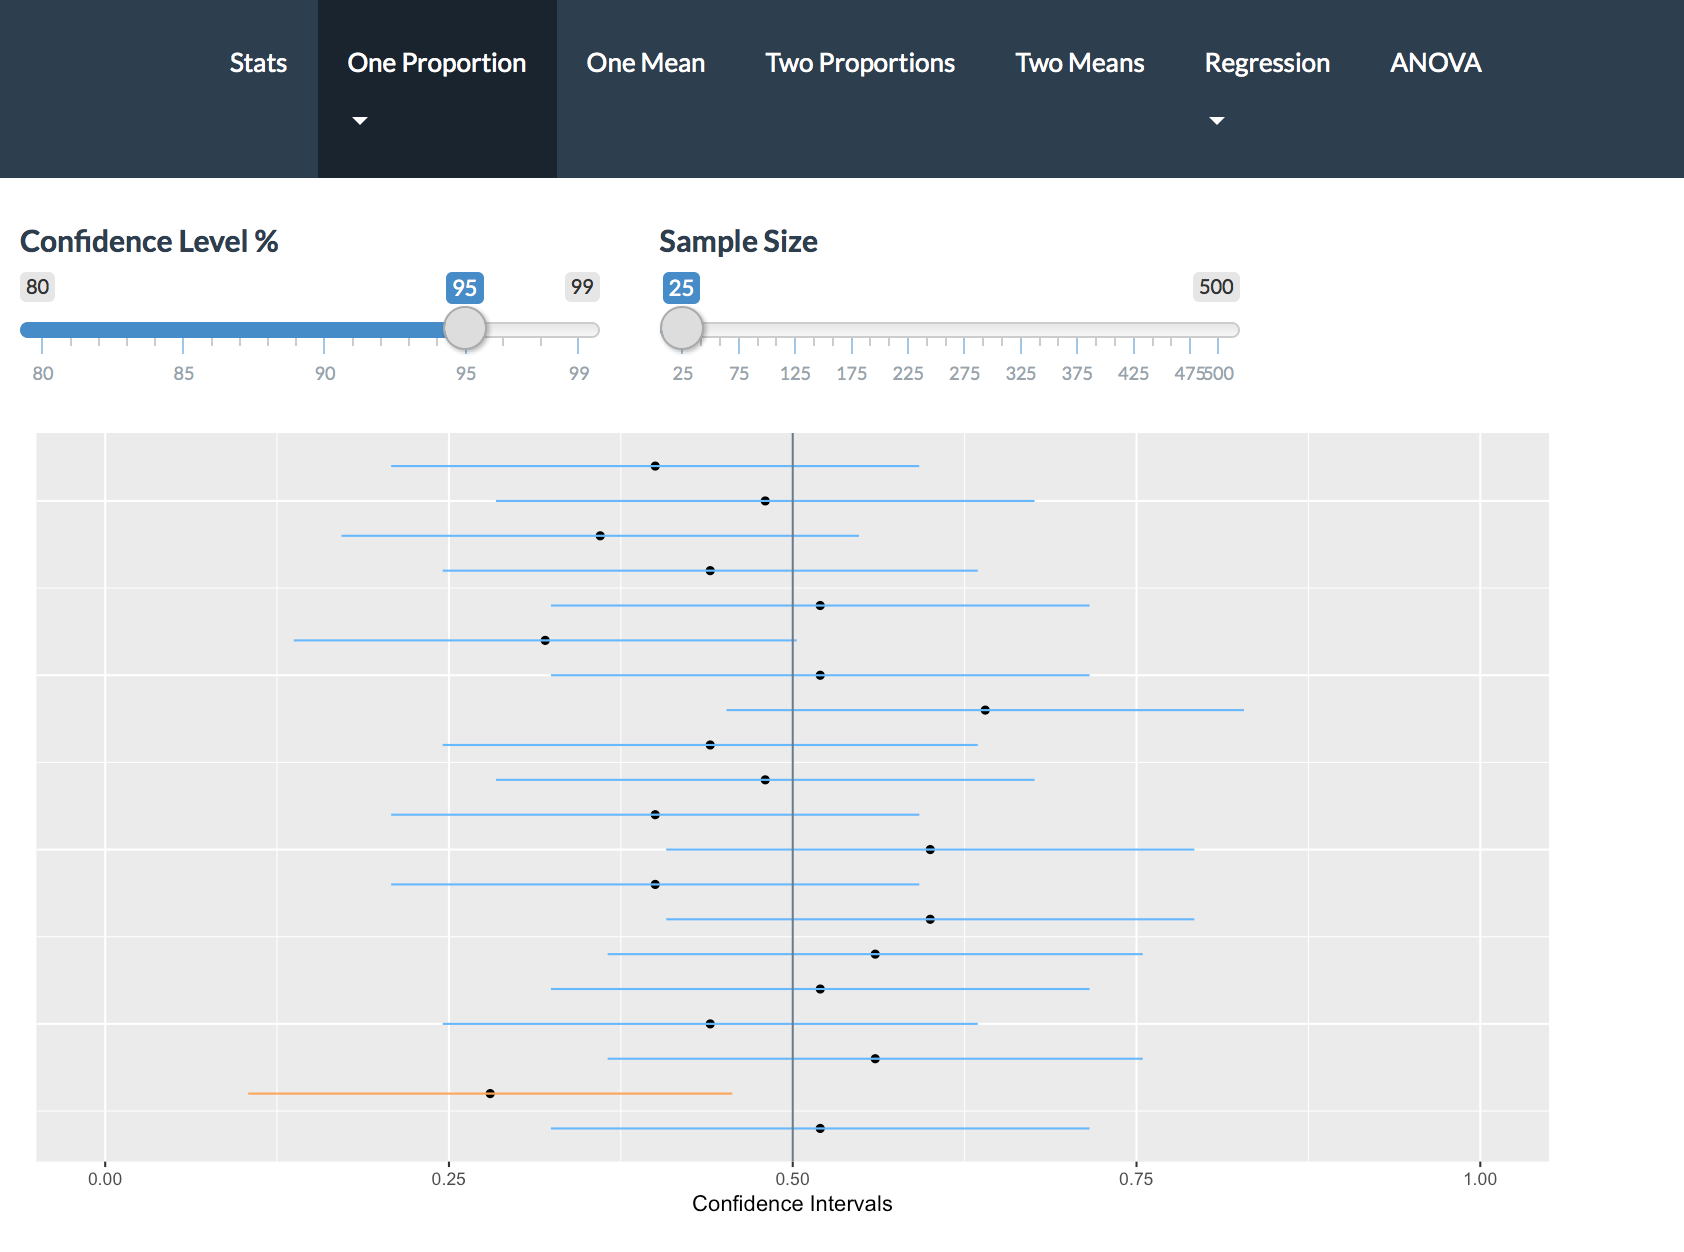
\includegraphics[width=\textwidth]{OnePropCI.png}
                \caption{Confidence Interval Screen} 
                \label{fig:OnePropCI}
        \end{subfigure}

\caption {Subsection of Inference for One Proportion}
\end{figure}

\newpage
\subsection{One Mean}
The section One Mean focuses on the concept of sampling distribution for one mean. The layout is similar to that of the sampling distribution for one proportion tab.  The user can enter the population mean, population standard deviation, sample size, and number of samples.  Once the "Draw" button is clicked, the sampling distribution of the sample mean appears with summary statistics (mean and Standard deviation) in addition to the last drawn sample distribution and its summary statistics (mean and standard deviation). All samples are drawn from a normal distribution with the mean and standard deviation input by the user.   We can see a screen shot of this section in Figure \ref{fig:OneMean}.

\begin{figure}
\centering
        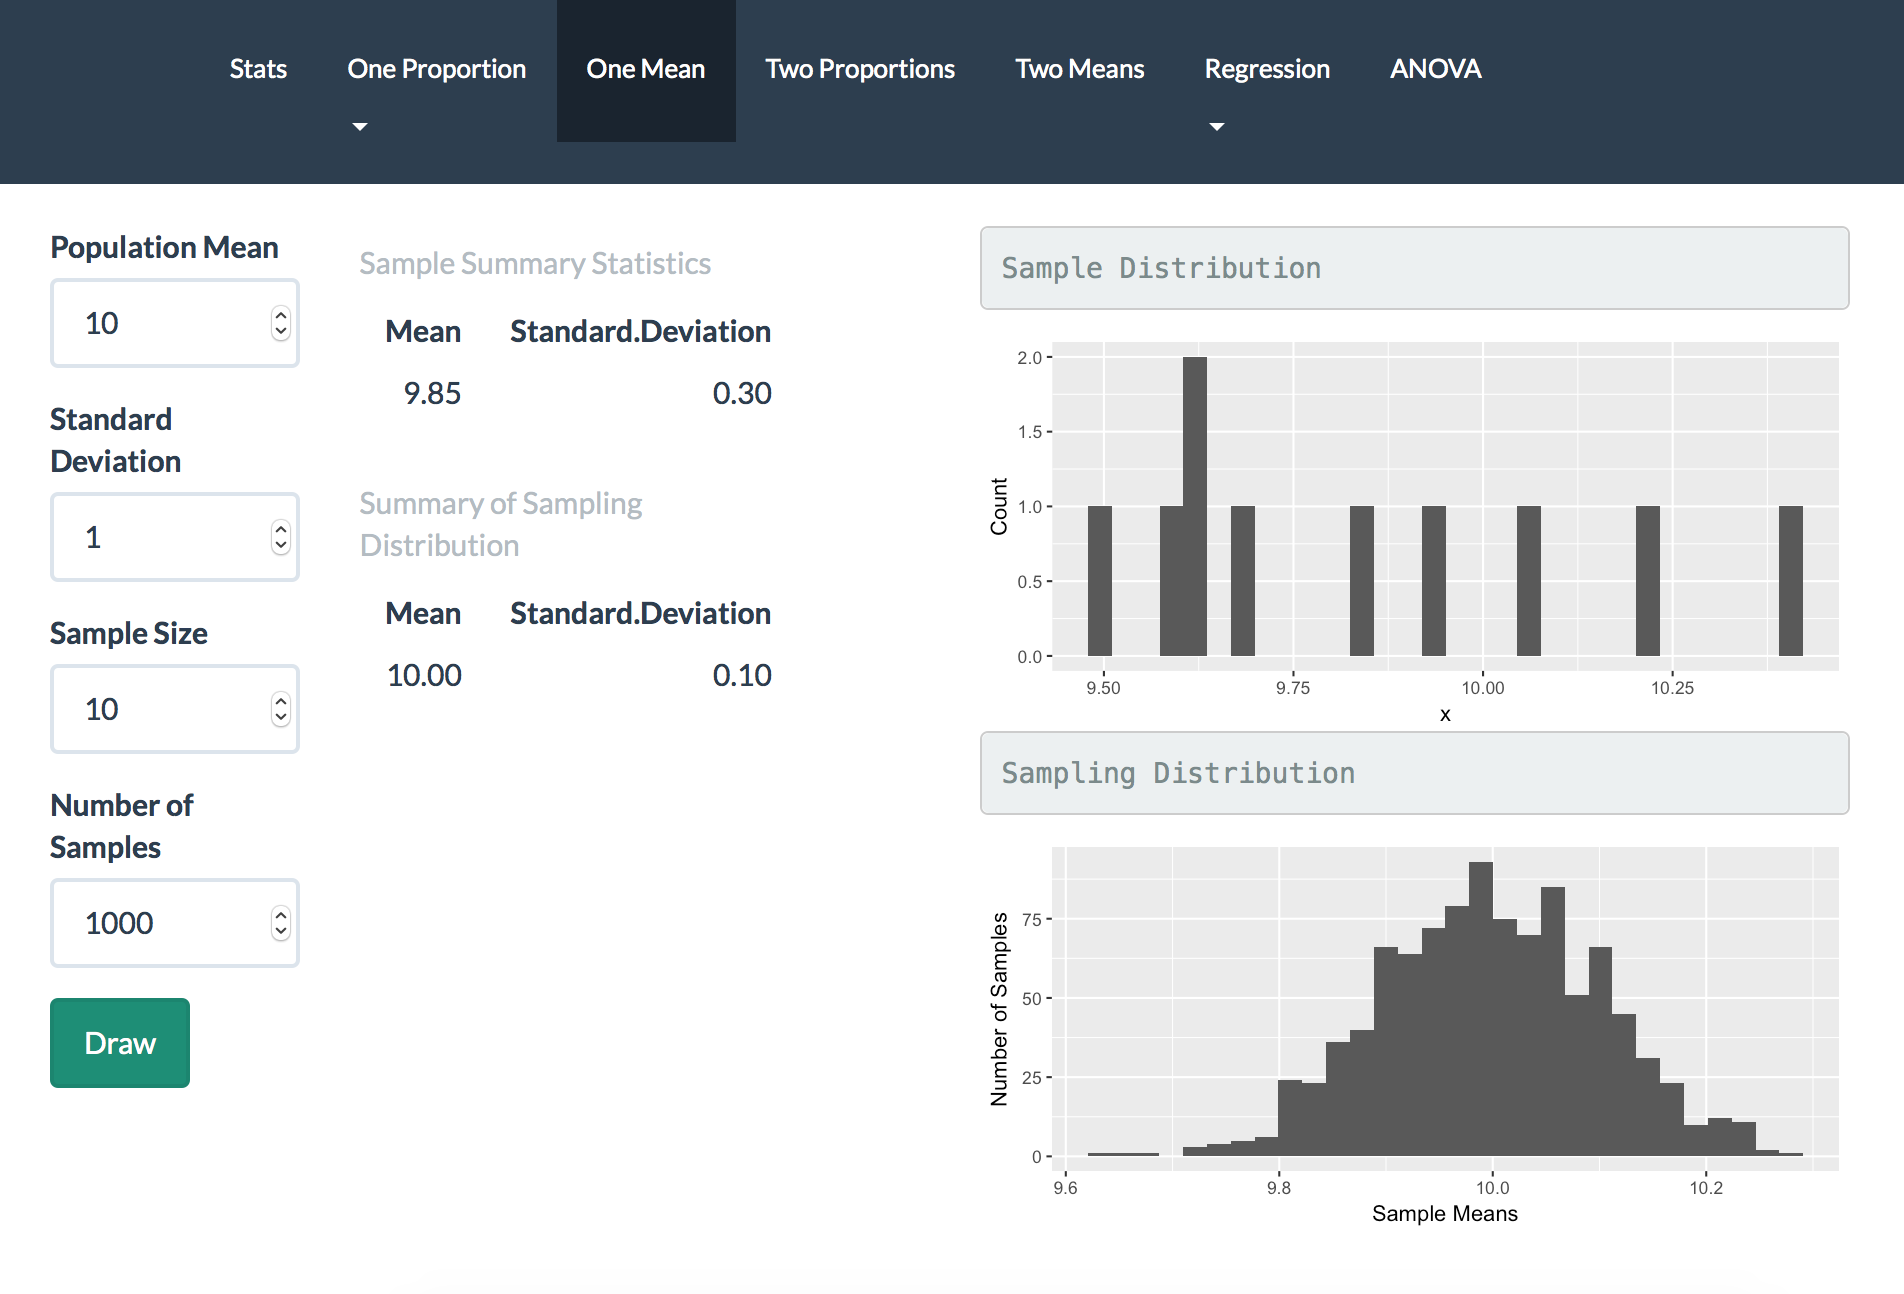
\includegraphics[width=\textwidth]{OneMean.png}
        \caption{One Mean}
        \label{fig:OneMean}
        
\end{figure}

\subsection{Two Proportions and Two Means}

The sections for two proportions and two means are constructed similarly to the single proportion and single means sections, as seen in Figure \ref{fig:TwoProp}.  They each aim to display the sampling distribution of the difference in the two sample statistics. The two proportions tab allows the user to input the population proportion for two different groups, the sample sizes for those groups, and the number of samples they wish to draw. The samples are then drawn from binomial distributions with the specified sample size and proportion for each group. The results of both samples are shown in the Sample Distribution graphs. The table of Sample Summary information displays the sample proportion for each group as well as the difference in those proportions. The Sampling Distribution graph is created by repeating this process many times and saving the differences in the two proportions each time. The summary information for the Sampling Distribution (mean and standard deviation) is displayed in the Sampling Distribution Summary table.

The Two Means tab recreates the same process except with calculating the difference in the two sample means for the two groups. The user can input a specific population mean, population standard deviation, and sample size for each of the two groups. The samples will then be generated from a normal distribution with those values. The results are similar to that of the two proportions tab, where the Sample Distribution graphs and Sample Summary information displays the sample mean for each group as well as the difference in the two means and the Sampling Distribution of the difference in the sample means is displayed along with the Sampling Distribution Summary table (mean and standard deviation). 

\begin{figure}
\centering
        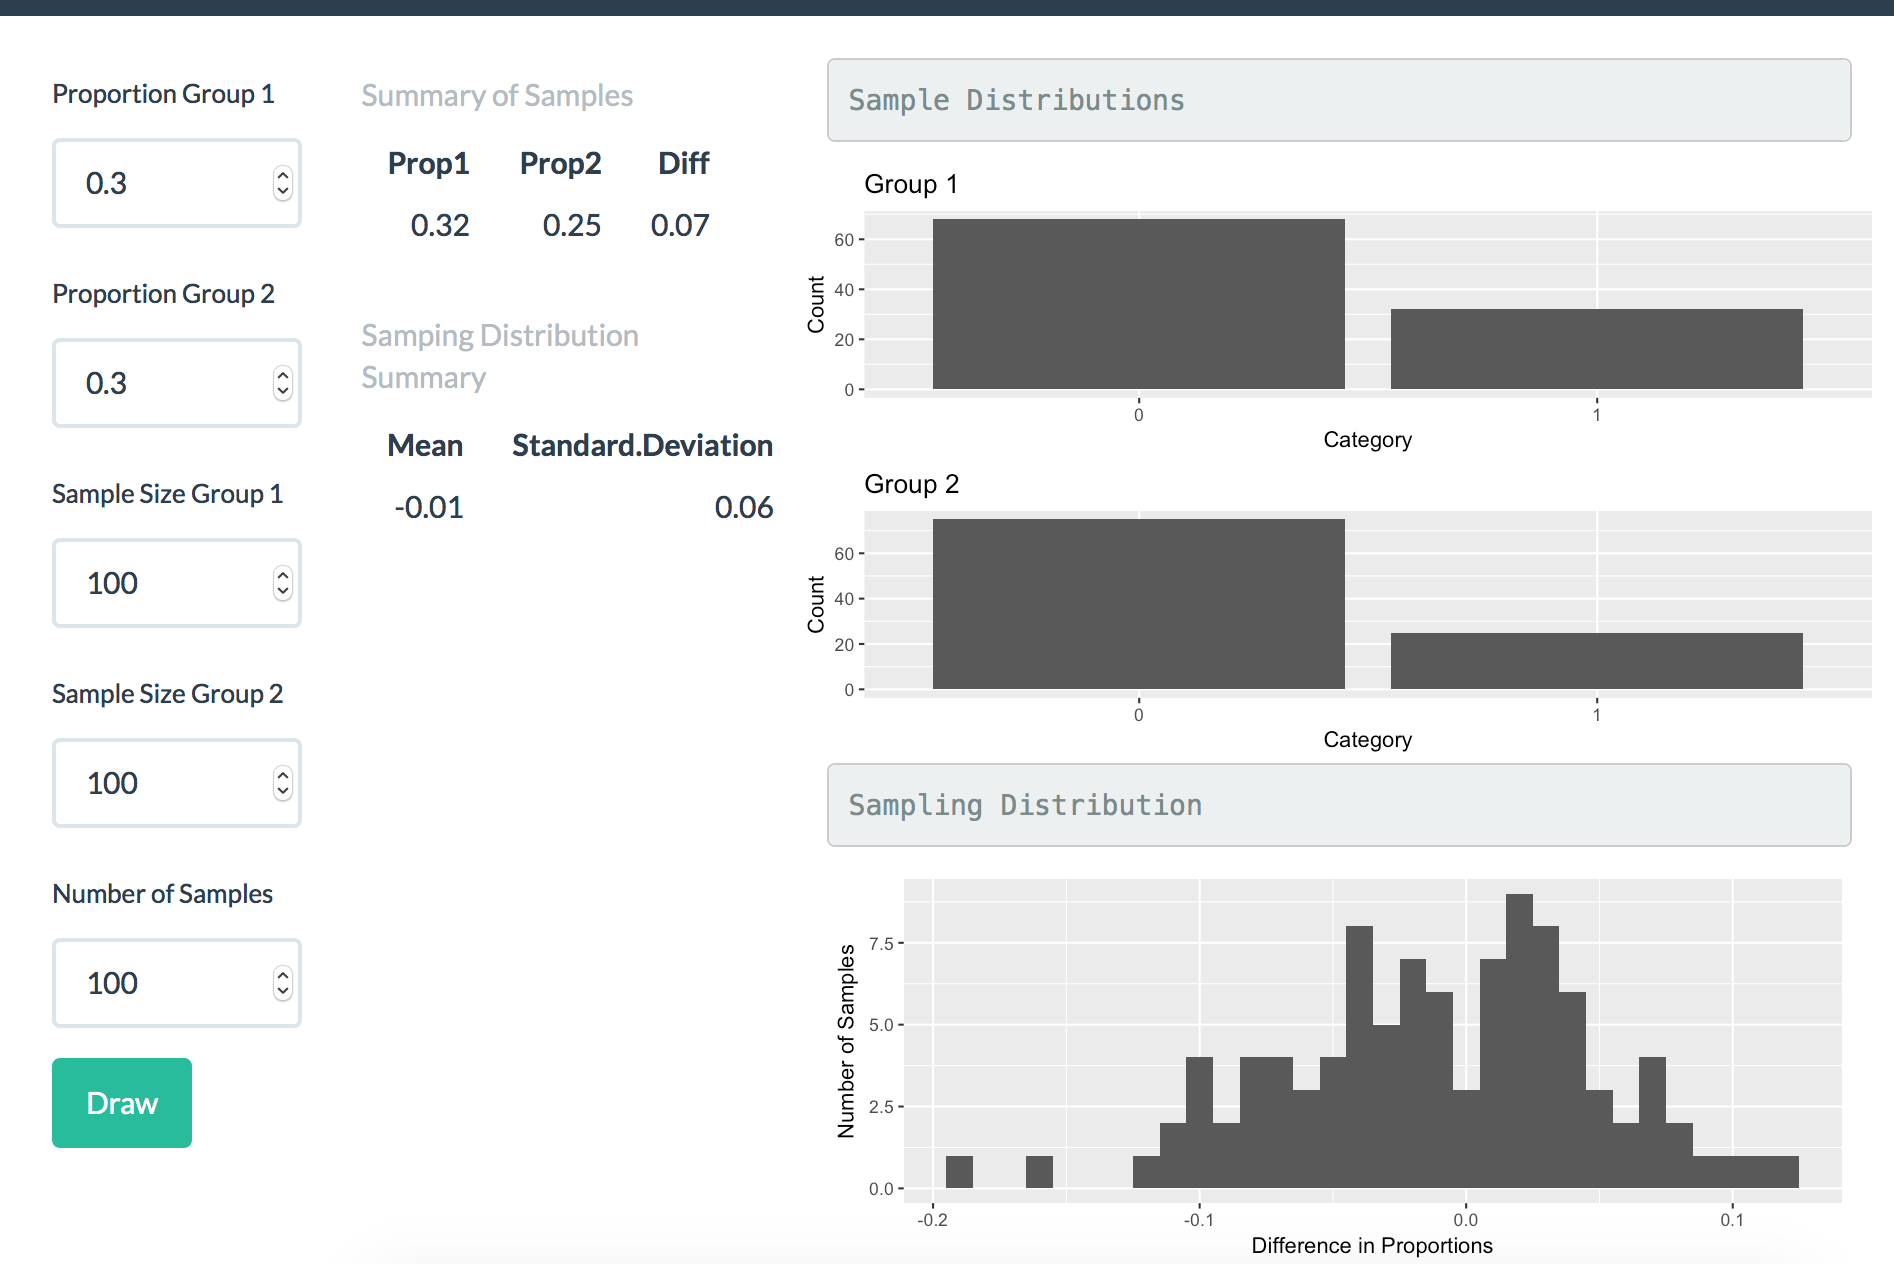
\includegraphics[width=0.75\textwidth]{TwoProp.png}
        \caption{Two Proportions} 
        \label{fig:TwoProp}
\end{figure}

\subsection{Linear Regression: Correlation}
Another section featured in the Shiny app is based on descriptive linear regression topics. The correlation page features a slider that allows the user to select correlation values for a random plot of points. Figure \ref{fig:Correlation} gives a screen shot of this section of the Shiny app with a user-specified correlation value of 0.73. The app allows the user to see what different correlations look like ranging from -1 to 1. In order to make this plot, a multivariate normal random data frame is created that has 100 sets of data points designed with a specific sigma matrix.  This sigma matrix changes based on the user input correlation value, but keeps 1 as the variance for both x and y.  Thus, the XY coordinates are generated with the set user-specified correlation. These points are then plotted on the graph and updated as the slider is moved. 

\subsection{Linear Regression: Outliers}
 
The outliers tab under Linear regression is designed to display multiple data sets with different types of outliers. The data sets are all identical except for the one outlier point, which will be set in a red color.  Once a data set is selected the user can select to fit a least squares regression line to the data, both with and without the outlier. Once the box is checked to fit a line to the data, the line is placed on the graph, blue for the line fit with the outlier and green slashes for the line fit to the data without the outlier. The output will also display the intercept, slope and coefficient of determination ($R^2$) for the lines on the graph.  
 
\subsection{Linear Regression: Equation}

The Equation section of the Shiny app breaks down the components of the least squares regression equation and provides interpretations for intercepts and slopes.  In addition, the user can manipulate the intercept and slope of the points on the graph in order to see how it changes the points and the line fit to them.  The data for this plot is generated using the same multivariate random normal data generating function in R as in the correlation section. In order to obtain a positive definite covariance matrix, the variance of $X$ is set to 1, the variance of $Y$ is set to 1000, and the input slope value is set to the covariance in the sigma matrix. The data is then adjusted to meet the intercept requirements by shifting the points created with the specific slope to pass through the user input intercept value. The data on the plot will update as the intercept and slope sliders are moved.  When the  ``Fit Line'' box is selected the equation for that least squares line will be displayed. It will have the same intercept and slope as the sliders display. The user can then select the ``Intercept" box to see a red dot appear at the y-intercept on the plot. They will also be shown an intercept interpretation that is specific the the intercept they see in the plot. Similarly, when the ``Slope" box is checked there is an interpretation of the slope that is output for the user.  The graph will display the rise and run of the slope to help illustrate the interpretation for the slope. A horizontal green line represents the one unit increase in the explanatory variable, while a vertical blue line indicates the average increase or decrease in the response variable as a result of the increase in the explanatory variable. The user can manipulate the sliders and the check boxes as they see fit, and the plot and output will continually update. Figure \ref{fig:LinEq} displays the screen for Equation when all boxes are checked. 


\begin{figure}
        \centering
         \begin{subfigure}[b]{0.6\textwidth}
                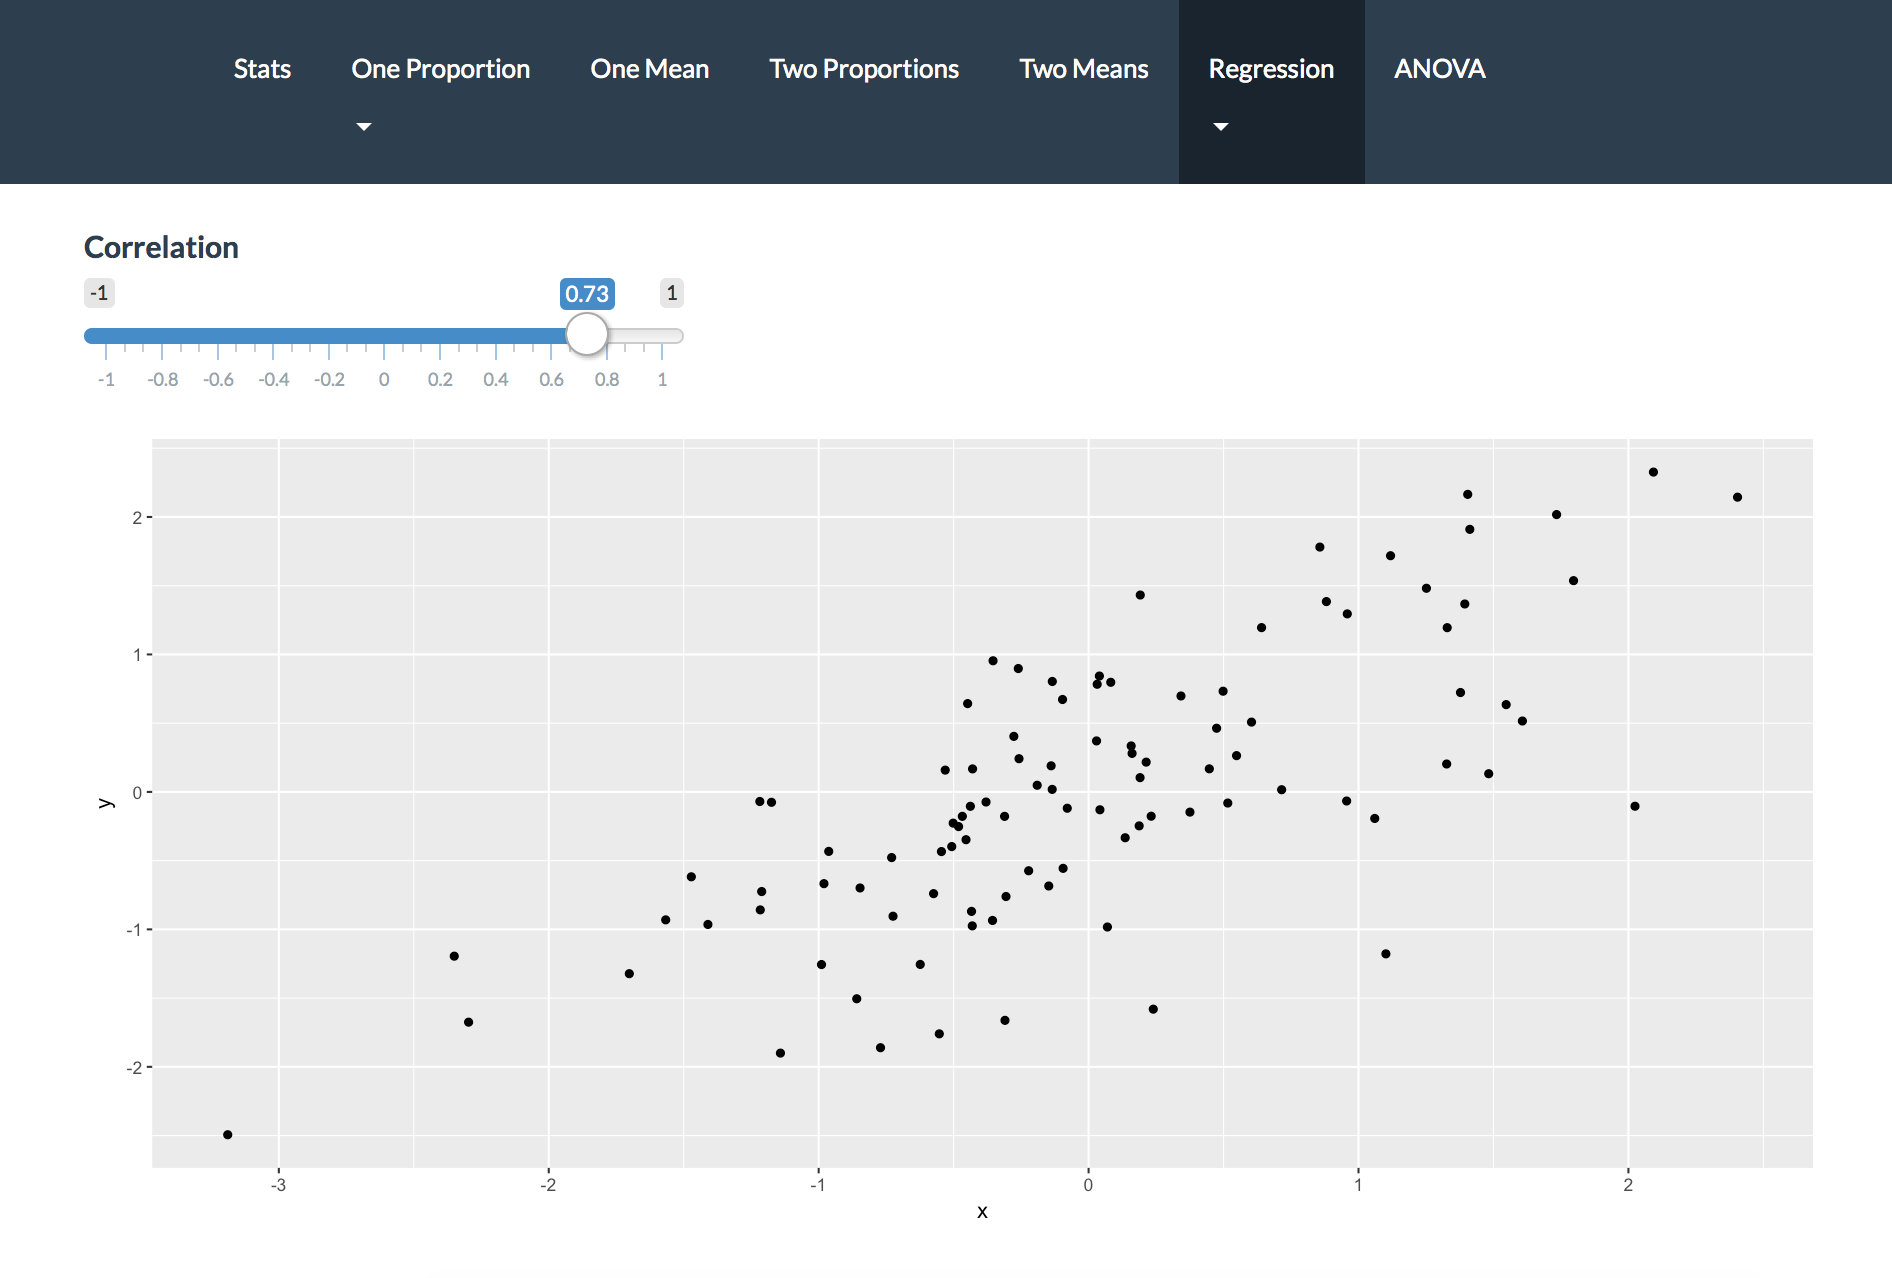
\includegraphics[width=\textwidth]{Correlation.png}
                \caption{Regression: Correlation} 
                \label{fig:Correlation}
        \end{subfigure}
        
        \begin{subfigure}[b]{0.6\textwidth}
                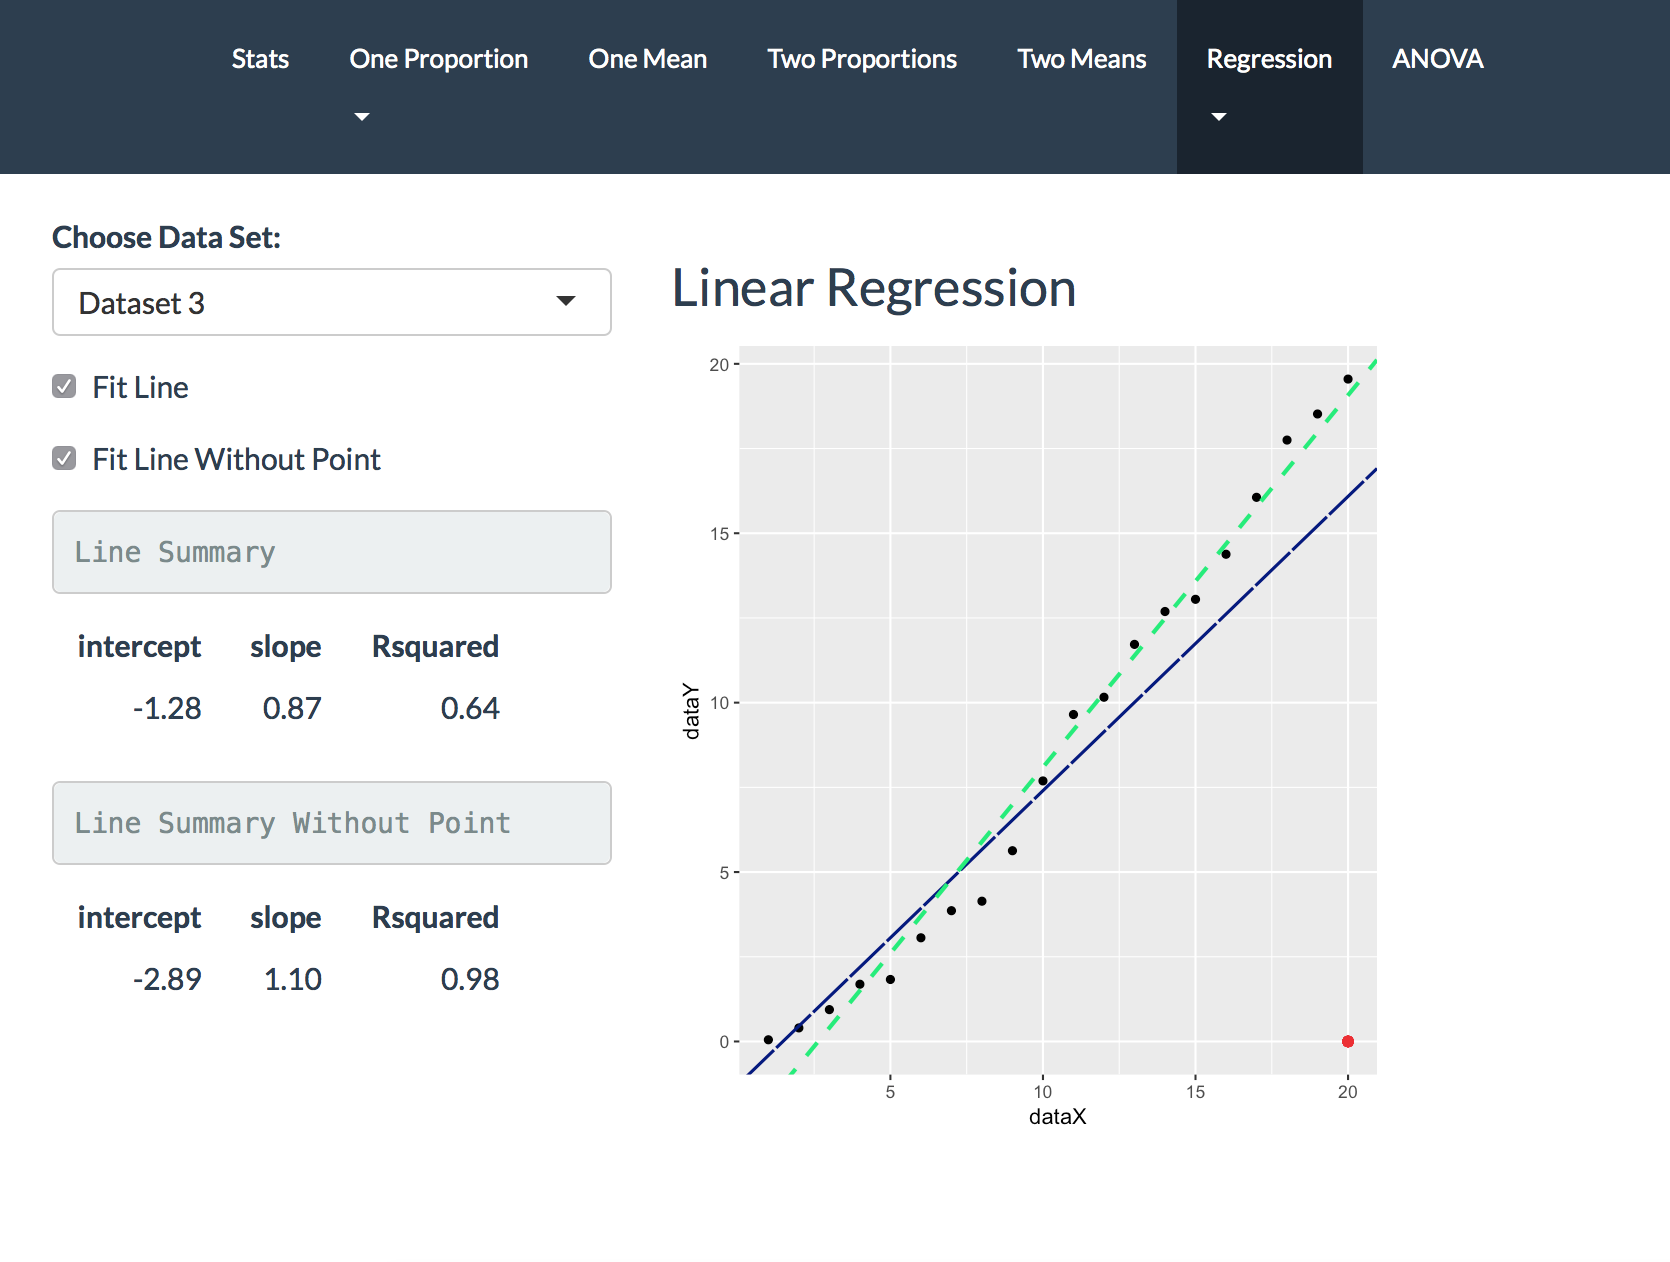
\includegraphics[width=\textwidth]{Outliers.png}
                \caption{Regression: Outliers }
                \label{fig:Outliers}
        \end{subfigure}%

        \begin{subfigure}[b]{0.6\textwidth}
                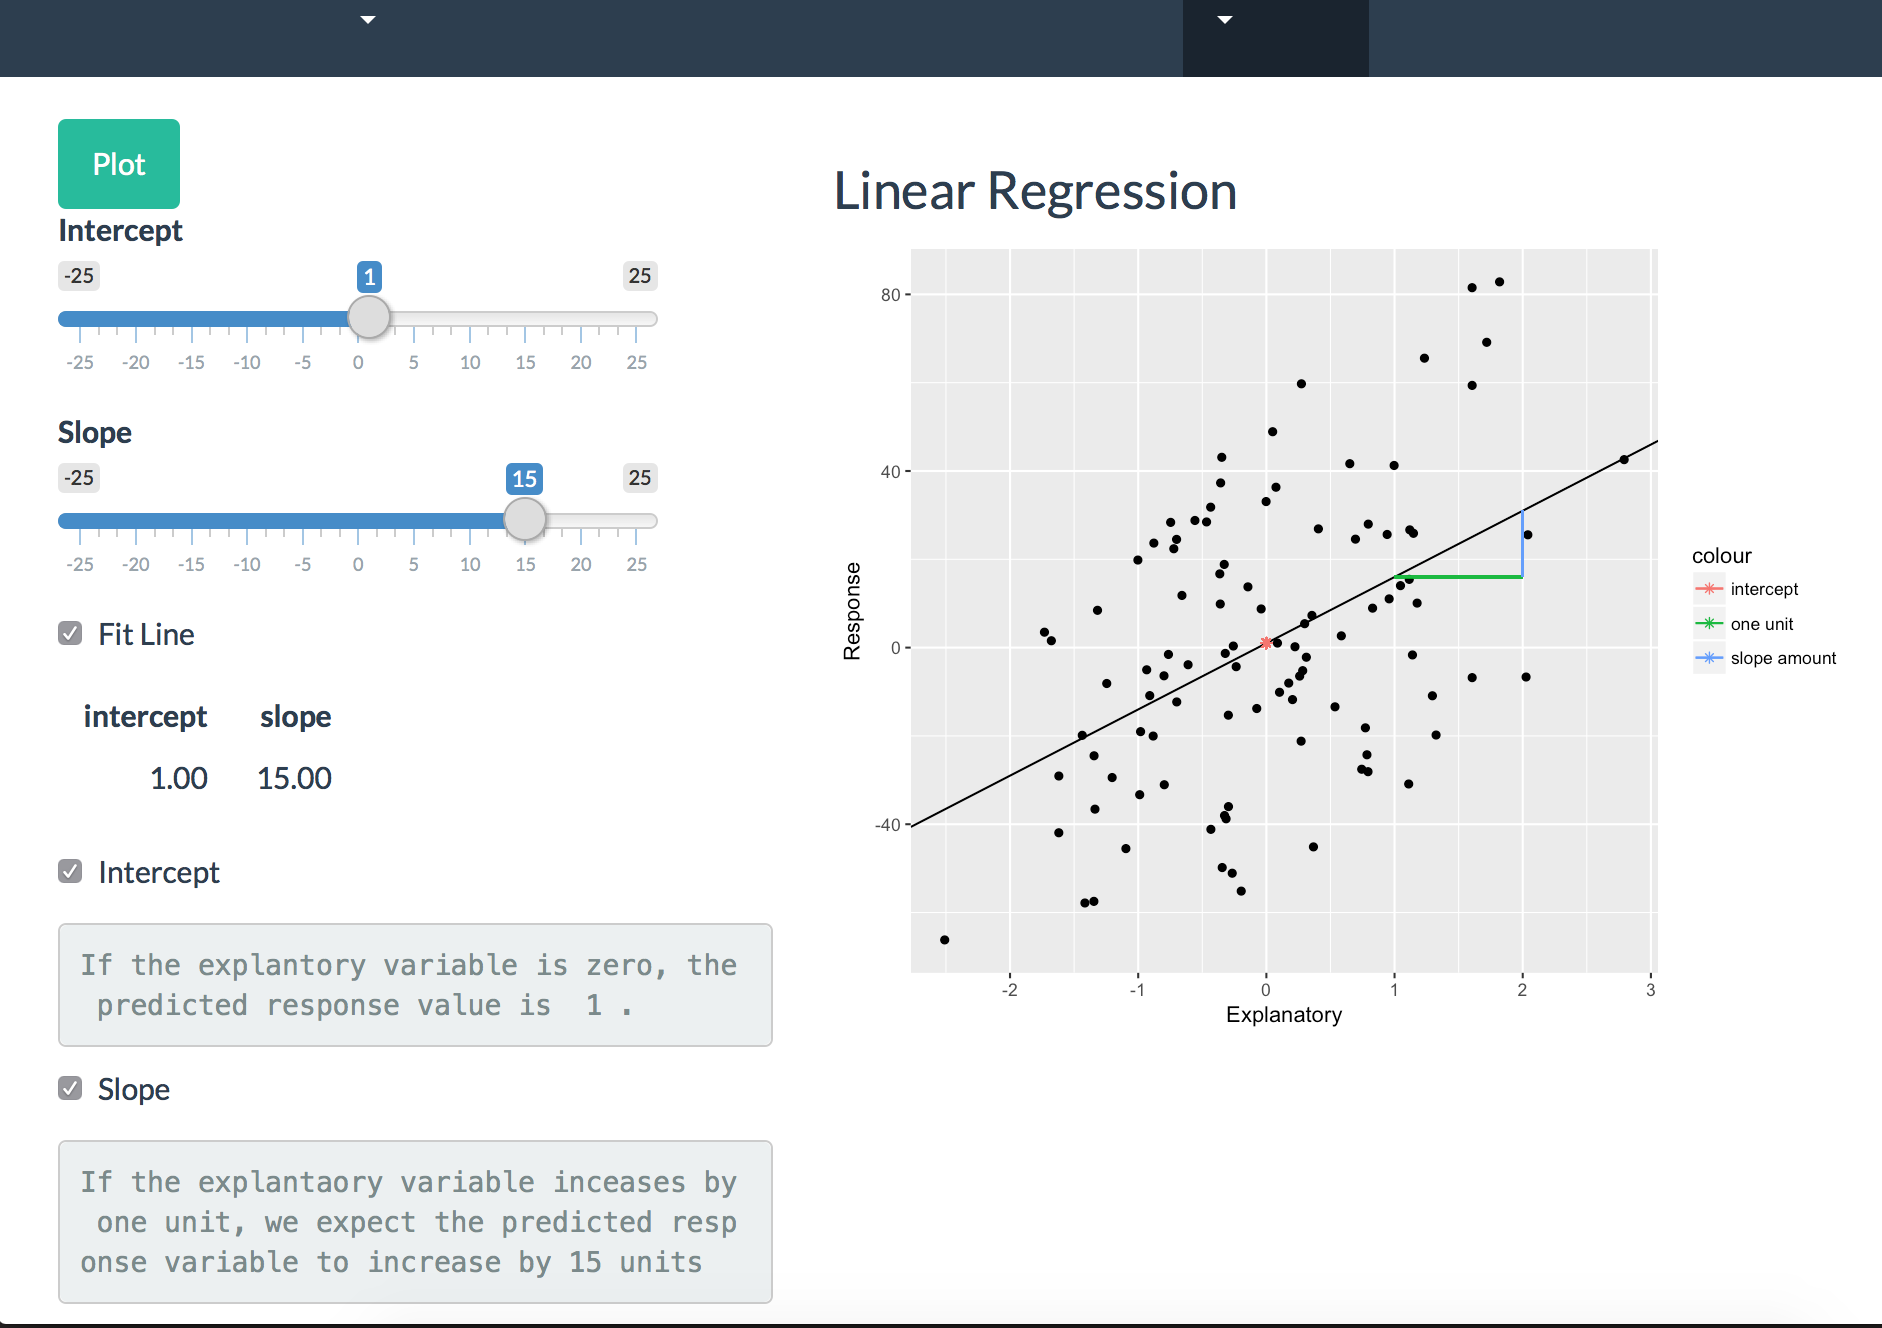
\includegraphics[width=\textwidth]{LinEq.png}
                \caption{Regression: Equation} 
                \label{fig:LinEq}
        \end{subfigure}
        

\caption {Regression Subsections}
\end{figure}

\subsection{ANOVA}

The last tab of the shiny application is the ANOVA tab.  This tab explores the relationship among the means of 3 different groups.  The user can input the population means, population standard deviations, and sample sizes for each of the three groups. This can be seen in Figure \ref{fig:ANOVAUP}. The samples are then generated for each group using a normal distribution with the each groups input values. The results include a dotplot of the sample distribution for each of the groups along with summary information and the ANOVA table for the difference in the sample means. The output for this part of the Shiny app can be seen in Figure \ref{fig:ANOVALOW}.

\begin{figure}
        \centering

        \begin{subfigure}[b]{0.75\textwidth}
                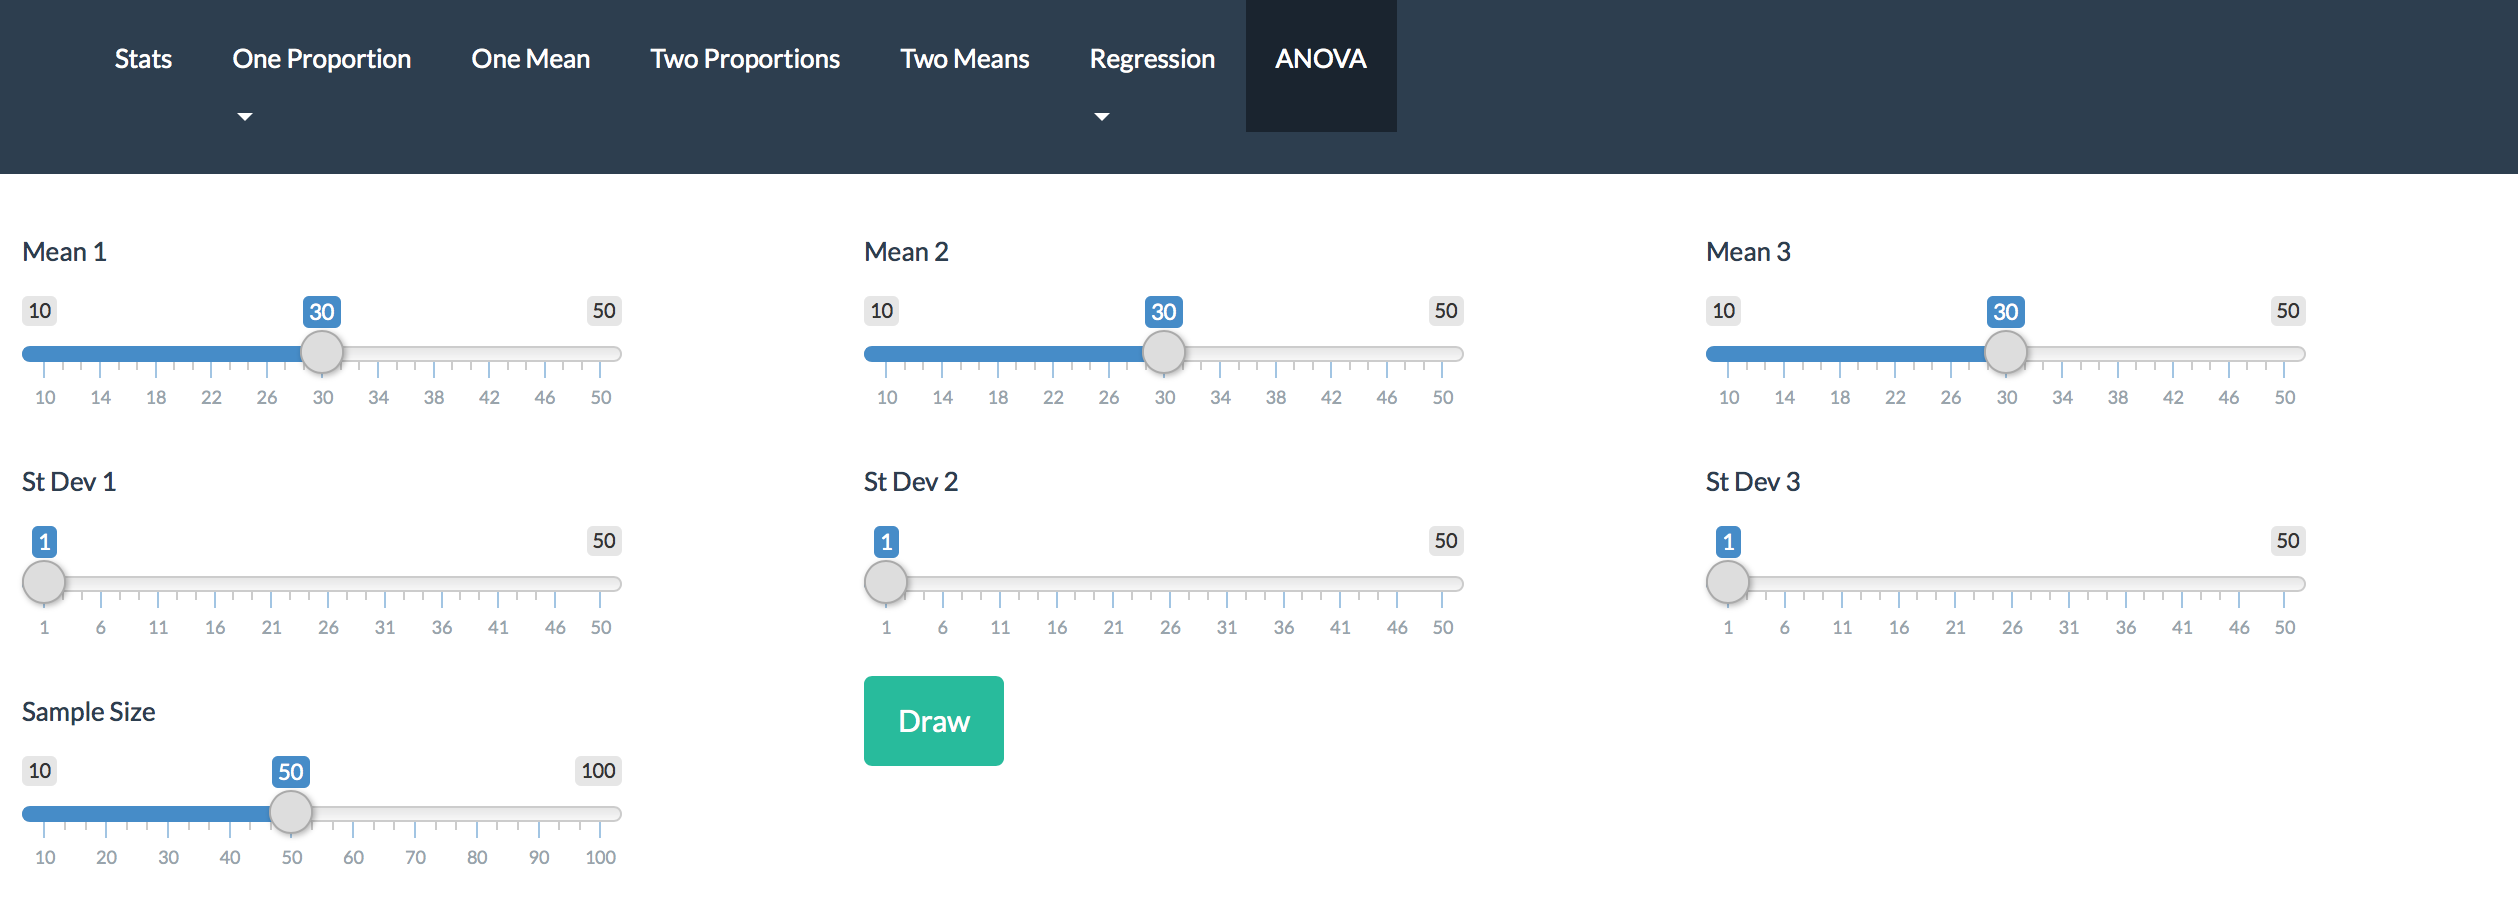
\includegraphics[width=\textwidth]{ANOVAUP.png}
                \caption{ANOVA Section top }
                \label{fig:ANOVAUP}
        \end{subfigure}%

        \begin{subfigure}[b]{0.75\textwidth}
                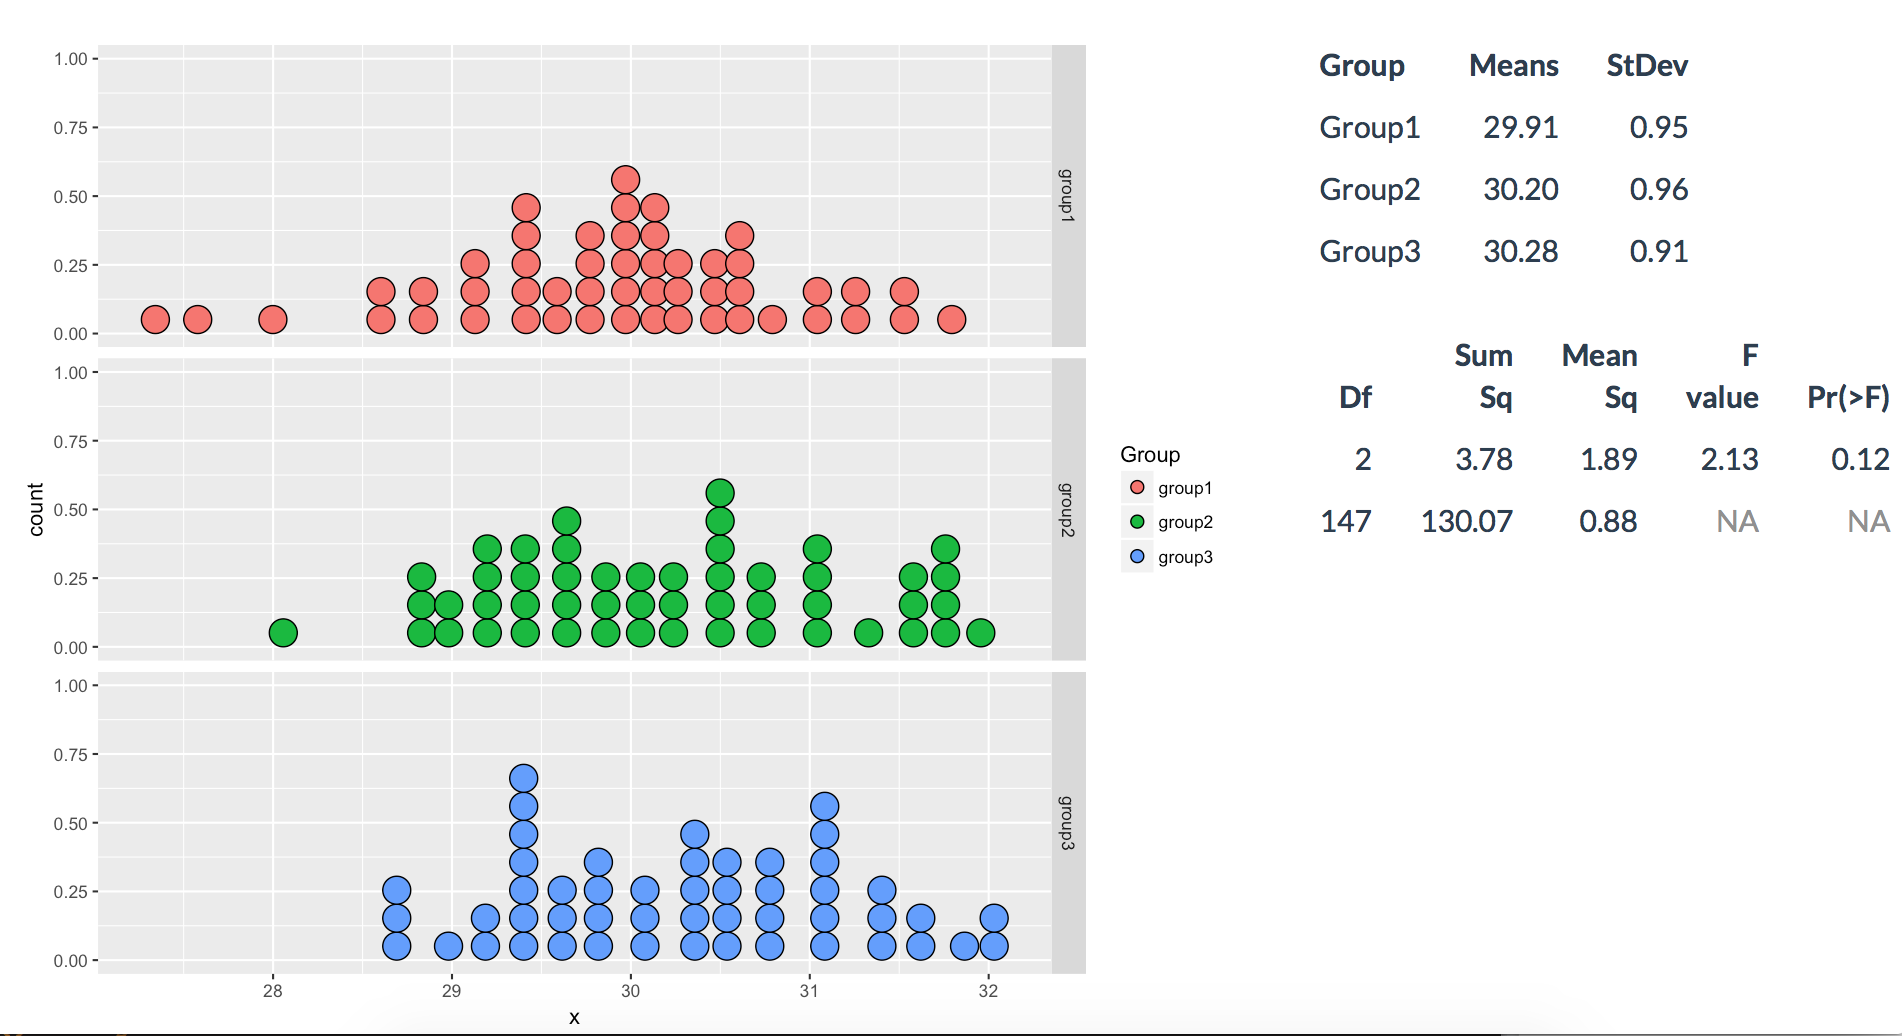
\includegraphics[width=\textwidth]{ANOVALOW.png}
                \caption{ANOVA Section lower} 
                \label{fig:ANOVALOW}
        \end{subfigure}

\caption {ANOVA Sections}
\end{figure}

\section{Supplemental Worksheets}

While the Shiny app could stand alone, we believe software developers should also focus their attention on developing learning materials to be used in conjunction with their programs. Along these lines, worksheets have been developed that illustrate to the user the important concepts in each section of the app. Below is an explanation of the concepts the worksheets cover for each section, along with the questions. 

\begin{itemize}
\item {\bf One Proportion: Sampling Distribution} The questions on the worksheet are designed to lead the user through drawing one sample and seeing how the results are displayed in the Sample Distribution vs in the Sampling Distribution. Then, the user is directed to drawing multiple samples with the goal of discovering the properties of the Sampling Distribution of the sample proportion (centered around the population proportion $p$, standard deviation approximately equal to $\sqrt{\frac{p(1-p)}{n}}$ and shape approximately normally distributed for large sample sizes.

\begin{enumerate}
\item Take one sample of size 100 with a population proportion of 0.3. Draw a graph of the sample distribution, and write the proportion of those chosen belonging to the ``yes" category. Note that the sampling distribution has one single bar at the value for the ``yes" proportion.

\item Now take 100 samples of size 100 with a population proportion 0.3.  How would you describe this sampling distribution (shape, center and variability)? 

\item Now take 1000 samples of size 100 with a population proportion of 0.3.  How would you describe this sampling distribution (shape, center and variability)?  

\item How do your answers for 2 and 3 above compare?
\end{enumerate}

\item {\bf One Proportion: Confidence Interval} This worksheet walks the user through fixing the confidence level and seeing what happens to the width of the intervals as the sample size in increased from 25 to 500. In the second question the sample size is fixed at 250 and the confidence level is increased from 80 to 99$\%$.  Through manipulation of these two components, the user is quickly able to see the relationship between confidence interval width, the sample size, and the confidence level.

\begin{enumerate}
\item Draw samples at confidence level 95$\%$, increasing the sample size from 25 to 500 slowly. What do you notice about the length of the intervals as the sample size increases? Why?

\item Now increase the confidence level from $80\%$ to $99\%$ slowly, keeping the sample size at 250. What do you notice about the length of the intervals as the confidence level increases? Why?

\end{enumerate}

\item {\bf One Mean} The questions on the worksheet are designed to lead the user through drawing one sample and seeing how the results are displayed in the Sample Distribution vs in the Sampling Distribution. Then, the user is directed to drawing multiple samples with the goal of discovering the properties of the Sampling Distribution of the sample mean (centered around the population mean $\mu$, standard deviation approximately equal to $\frac{\sigma}{\sqrt{n}}$ and shape normally distributed.  

\begin{enumerate}
\item Take 1 sample of size 25 with a population mean of 20 and a standard deviation of 3. Draw a graph of the sample distribution, and write the mean of your sample. Note that the sampling distribution has one single bar at the value of the mean for your sample.

\item Take 100 samples of size 25 with a population mean of 20 and a standard deviation of 3.  What do you notice about the sampling distribution now?

\item Take 1000 samples of size 25 with a population mean of 20 and a standard deviation of 3.  How would you describe this sampling distribution? What is the mean for this sampling distribution?

\end{enumerate}

\item {\bf Two Proportions and Two Means} This worksheet leads the user through taking multiple samples to build the sampling distribution of the difference in the two sample statistics, which ends up being approximately normal, similar to the one proportion and one mean inference sections.

Two Proportions

\begin{enumerate}
\item Set the proportion for group 1 to 0.3 and the proportion for group 2 to 0.4. Also, set the number of samples to 1, and draw a sample. What $\hat{p}$ for each sample? 

\item What is your sample statistic for the difference in proportions from question 1?

Note: The sampling distribution has one sample at your sample difference in proportions value.

\item Set number of samples to 100 and redraw. Describe the shape, center, and symmetry of your sampling distribution. 
\end{enumerate}

Two Means
\begin{enumerate}
\item Draw 1 sample with sample size 50 for each group. Set group 1 mean to be 20 and group 2 mean to be 21.  Let the standard deviations for both be 1. What are your sample means for each group?

\item What is your sample statistic for the difference in means from question 1? Note: The sampling distribution has one sample at your sample difference in means value.

\item Set number of samples to 100 and redraw. Describe the shape, center, and symmetry of your sampling distribution. 
\end{enumerate}
  
\item {\bf Correlation} The questions on the worksheet guide the user through observing the layout of the scatterplot as the slider moves from a correlation of -1 to 1. They will take note of the direction and form of the relationship as the correlation changes. 

\begin{enumerate}
\item Set the correlation to -0.9. Describe the form, strength, and direction of the points.

\item Set the correlation to -0.5. Describe the form, strength, and direction of the points.

\item Set the correlation to 0.5. Describe the form, strength, and direction of the points.

\item Set the correlation to 0.9. Describe the form, strength, and direction of the points.

\item What do you notice about the form and strength as you increased the correlation from -0.9 to 0.9?
\end{enumerate}

\item {\bf Outliers} The worksheet leads the user through the linear model selection process of fitting data both with and without an outlier and determining the effect of the outlier on the model. Users will also look at multiple outliers and determine whether they have high leverage, high residual or both.

\begin{enumerate}

\item Select "Dataset 1", and observe the point in red. Click "Fit Line" to get a least squares line to the data. Write the equation of the line below.

\item Next, remove the red point and refit the least squares line by checking the "Fit Line Without Point" box.  Write the equation for that line below. 

\item Do you think that fitting the data without the red point improved the fit of the line to the data? Why?

\item Select "Dataset 2", and observe the point in red. Click "Fit Line" to get a least squares line to the data. Write the equation of the line below.

\item Next, remove the red point and refit the least squares line by checking the "Fit Line Without Point" box.  Write the equation for that line below. 

\item Do you think that fitting the data without the red point improved the fit of the line to the data? Why?

\item Choose "Dataset 3" from the dropdown. Fit the least squares regression line both with and without the red outlier. Do you think the point has high leverage? Do you think the point has a large residual? Explain.

High leverage:

Large residual:

\item Choose "Dataset 4" from the dropdown. Fit the least squares regression line both with and without the red outlier. Do you think the point has high leverage? Do you think the point has a large residual? Explain.

High leverage:

Large residual:

\end{enumerate}

\item {\bf Equation} The questions on the worksheet guide the user through manipulating the slope and intercept on the plot and providing interpretations of those values.

\begin{enumerate}
\item Set the intercept to -10 and the slope to 5. Click "Fit Line" and write the equation for the least squares regression line.

\item Write the y-intercept interpretation. Then, check the "Intercept" box and see if your interpretation is correct. Note, the red dot on the plot inidcation the location of the y-intercept.

\item Write the slope interpretation. Then, check the "Slope" box and see if your interpretation is correct.

\item Set the intercept to 20 and the slope to -15. Click "Fit Line" and write the equation for the least squares regression line.

\item Write the y-intercept interpretation. Then, check the "Intercept" box and see if your interpretation is correct.

\item Write the slope interpretation. Then, check the "Slope" box and see if your interpretation is correct. What is the difference between this interpretation and the one in number 3? Explain this difference.

\end{enumerate}
  
\item {\bf ANOVA} The worksheet gives the user a short introduction to the ANOVA F-test followed by some questions asking them to explore the relationship between the mean, standard deviation, sample size and the resulting p-value and conclusion of the F-test. 

\begin{enumerate}
\item Set all means to 30 and all standard deviations to 1.  State the p-value and conclusion for a test of difference in means.

\item Set the means to 20, 30, and 30 respectively.  Set all standard deviations to 5.  Draw a sample and state the p-value and conclusion.  

\item Set the mean for groups 1 and 2 to 30, and mean of group 3 to 32.  Set all standard deviations to 5.  Take a sample with sample size 100 and note what the p-value is for the ANOVA test.  Write a conclusion based on your p-value.

\item Next, keep the settings the same as above, but draw a sample of size 10.  Note the p-value, and write a conclusion based on this p-value.  

\item What generalization can be made regarding sample size and test outcome after observing what happened in the previous questions?

\end{enumerate}

\end{itemize}

\section{Conclusions and Future Work}
Technology plays an important role in the design and structure of the modern introductory statistics course. Many current technologies have advantages and disadvantages to their use in the classroom. The purpose of this project was develop an R Shiny app to help students investigate concepts in introductory statistics. R's Shiny app technology provides a free, easy to use, customizable platform for educators of introductory statistics courses. The Shiny app outlined in this paper can easily be launched to the web and used in courses along with the supplementary worksheets. In addition, the flexibility of programming the Shiny app created here lends itself to be easily altered, based of the requirements of the course or instructors needs. As long as the instructor is familiar with R programming, new tabs or subsections can easily be added as needed, to be more specific to the course being taught. 

Future work is forthcoming on testing the software in the next few months. The Shiny app and a selection of the corresponding worksheets will be used on a sample of undergrads that have taken at least an introductory course in statistics and high school and community college mathematics teachers. Each group will answer a few opening questions about the concepts to be studied. Then, they will have the opportunity to use the Shiny app and work on the worksheets for two different sections. Then, there are another few questions for them to answer that correspond to the sections they worked on. Feedback will be collected from these groups on the software and improvements will be considered accordingly.  



\begin{thebibliography}{1}

\bibitem{chance}  Chance, B., Ben-Zvi, D.,$\&$ Garfield, J.,  Medina, E. (2007). The Role of Technology in Improving Student Learning of Statistics.

\bibitem{doi}  Doi, J., Potter G., Wong J., Alcaraz I., $\&$ Chi, P. (2016). Web Application Teaching Tools for Statistics Using R and Shiny. 

\bibitem{Pea} Roy D. Pea. Cognitive Technologies for Mathematics Education. A. Schoenfeld. Cognitive science and mathematics education. Hillsdale, pp.89-122, 1987. $<$hal-001990547$>$

\bibitem{Rossman} Rossman, A.$\&$ Chance, B. (2004), The \emph{Rossman/Chance Applet Collection}. Available at www.rossmanchance.com/applets.

\end{thebibliography}

\end{document}


